% Chapter 2

\chapter{L'environnement du stage} % Main chapter title

\label{environnement} % For referencing the chapter elsewhere, use \ref{Chapter1}

\lhead{Deuxième partie. \emph{L'environnement du stage}} % This is for the header on each page - perhaps a shortened title

%----------------------------------------------------------------------------------------
\section{Description de l'entreprise}
%----------------------------------------------------------------------------------------

\subsection{L'entreprise en général}
\begin{figure}[h]
  \centering
  
\includegraphics[scale=0.15]{Pictures/logoFC.jpg}
\end{figure}
FIGARO CLASSIFIEDS, filiale du GROUPE FIGARO, est une des sociétés Internet les plus importantes en France, avec 60 M\texteuro de C.A., 350 collaborateurs et 3,5 millions de visiteurs uniques dédupliqués par mois sur l’ensemble de leurs sites.
Anciennement connue sous le nom d'ADENCLASSIFIEDS, fusion des sociétés CADREMPLOI, KELJOB et EXPLORIMMO, cette société est depuis sa création dirigée par Thibault GEMIGNANI.
Elle est présente sur 3 gros secteurs: l’Emploi, la Formation et l’Immobilier et elle a pour ambition de proposer aux internautes et aux professionnels le meilleur des médias et des solutions d'annonces classées en France.
Ses marques-phares (CADREMPLOI, KELJOB, LE FIGARO ETUDIANT, EXPLORIMMO, PROPRIETES DE FRANCE…) allient puissance, affinité CSP+ et influence, comme autant de facteurs de différentiation par rapport à leurs concurrents.

FIGARO CLASSIFIEDS réalise 80\% de son chiffre d’affaires sur Internet, contribuant au développement numérique du GROUPE FIGARO, dont plus de 20\% du chiffre d’affaires total est réalisé sur Internet.

\subsubsection{Secteur d'activité}
% TODO concurrents, marché, évolution, ...
Le groupe est donc présent sur trois grand secteurs que sont l’Emploi, la Formation et l’Immobilier.
\paragraph{Emploi}
Pionnier du marché des annonces Emploi (print, web, mobile...), FIGARO CLASSIFIEDS propose une offre unique sur le marché, fondée sur une approche multi-marques et multi-produits, lui permettant d'être à tous les carrefours de rencontres entre candidats et recruteurs:
\begin{figure}[b]
  \begin{center}
    \hspace*{-1in}
    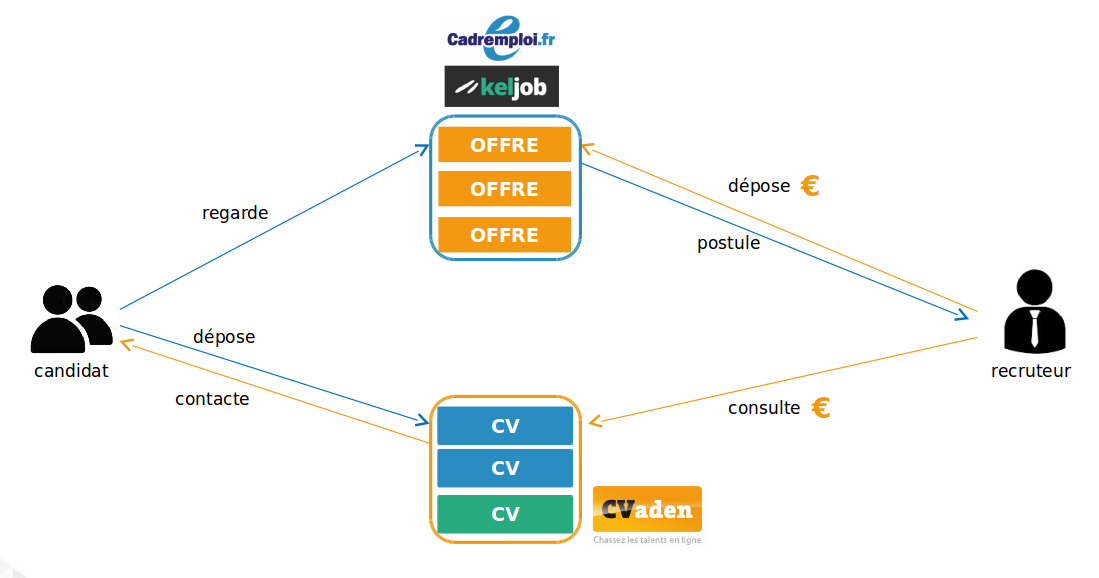
\includegraphics[width=1.25\textwidth]{Pictures/EmploiFCMS.png}
  \end{center}
\end{figure}
\begin{itemize}
  \item N°1 de l'Emploi privé sur Internet, avec les marques CADREMPLOI, KELJOB et CADRESONLINE
  \item N°1 de l'Emploi privé dans la presse nationale, avec LE FIGARO ECONOMIE
  \item N°1 de l'Emploi privé sur le Mobile, avec le succès des applications de CADREMPLOI et de KELJOB
\end{itemize}
Elle s'entoure aussi d'acteurs puissants dans le domaine de l'emploi, comme par exemple THE NETWORK, réseau international de recrutement N°1 (présent dans 136 pays).
Enfin, FIGARO CLASSIFIEDS se présente aussi comme un fournisseur de solutions RH, avec des produits comme CVAden (4 millions de CV), Adensourcing, CVmail ou Adenweb.

\paragraph{Formation}
Fort de son leadership et de son expertise sur le marché de l'Emploi, FIGARO CLASSIFIEDS a été l'un des pionniers sur le marché des annonces de formation sur Internet depuis 2004.
FIGARO CLASSIFIEDS peut ainsi accompagner les individus tout au long de leur carrière : formation initiale, en alternance, stages, recherche d'emploi, formation continue ou mobilité professionnelle via ses produits:
\begin{itemize}
  \item Le site Internet et l'application mobile de KELFORMATION
  \item Les rubriques « Formation » des sites CADREMPLOI, KELJOB et CADRESONLINE
  \item La CV-thèque Alternance de KELFORMATION
  \item Les titres de presse LE FIGARO, LE FIGARO ECONOMIE et LE FIGARO ETUDIANT
  \item La plateforme de vidéos CAMPUS CHANNEL
\end{itemize}

\paragraph{Immobilier}
À travers l'ensemble de ses médias, FIGARO CLASSIFIEDS dispose aussi d’une offre complète sur l’immobilier:
\begin{itemize}
  \item L’Ancien, avec EXPLORIMMO, PROPRIETES DE FRANCE, et LE FIGARO
  \item Le Neuf, avec EXPLORIMMONEUF
  \item Les Loisirs, avec BELLES MAISONS A LOUER
  \item Les Solutions, avec IMMOVISION (logiciel de transactions, référencement, digital agency…)
\end{itemize}

\subsubsection{Métiers}

On retrouve différents corps de métiers dans cette entreprise, puisque 5 grandes directions se côtoient:  Digital, Marketing, Communication et Édition, Ressources Humaines et Contrôle de Gestion.
Je faisais partie, en ce qui me concerne, du pôle Digital.

%----------------------------------------------------------------------------------------

\subsection{L'entreprise et son informatique}
L'informatique occupe une place très importante dans le département Digital de FIGARO CLASSIFIEDS.
Cette branche a majoritairement vocation a développer des applications web, c'est pourquoi de nombreux outils sont disponibles.

\subsubsection{Outils, technologies et méthodes}
\label{subs:Outils, technologies et methodes}
La plupart des employés a accès à un ordinateur, et un compte est attribué à l'arrivé, lui permettant de gérer notamment ses mails ou ses jours de congés.
Les développeurs sont pour la majorité sous Ubuntu et développent via l'IDE IntelliJ Idea pour lequel une license est disponible.
L'utilisation de l'ordinateur à disposition est plutôt libre, puisqu'il est permis d'installer des logiciels sans avoir à passer par des Demandes de Prestation Informatique.
La majorité des équipes échelonne sa mise en production sous plusieurs étapes en déployant une nouveauté sur des serveurs internes particuliers avant de procéder au déploiement public.
Cela permet de sécuriser les nouvelles versions du logiciel puisqu'il est ainsi possible de s'apercevoir d'un problème avant qu'il ne soit visible par le public.

\subsubsection{Outils de travail collaboratifs}
\label{subs:Outils de travail collaboratifs}
Des outils sont aussi disponibles pour permettre aux équipes de travailler ensemble plus facilement.
\paragraph{Redmine}
\label{par:Redmine}
\begin{wrapfigure}{l}{0.3\textwidth}
  \begin{center}
    
\includegraphics[width=0.20\textwidth]{Pictures/redmine_logo.png}
  \end{center}
\end{wrapfigure}
Redmine est un logiciel de gestion de projet qui est utilisé chez Figaro CLASSIFIEDS pour notamment lister les demandes client et qui permet de rendre compte en ligne du travail effectué.
Lorsque l'on s'occupe d'une tâche, qu'on la termine ou que l'on a besoin de plus de renseignement, on le mentionne sur Redmine, ce qui permet de centraliser l'information et de la rendre disponible au reste de l'équipe.
\paragraph{Git}
\label{par:Git}
\begin{wrapfigure}{r}{0.3\textwidth}
  \begin{center}
    
\includegraphics[width=0.30\textwidth]{Pictures/git_logo.jpg}
  \end{center}
\end{wrapfigure}
Git est un outil de gestion de versions.
Il est aussi utilisé au sein du pôle Média pour mettre en commun le code écrit par toute l'équipe.
Il s'agit d'un outil que j'avais déjà beaucoup utilisé à l'EISTI mais d'une façon très simpliste, et j'ai appris au cours de mon stage de nombreuses nouvelles possibilité d'utilisation pour cet outil que nous n'avions jamais exploité à l'école.
\paragraph{Slack}
\label{par:Slack}
\begin{wrapfigure}{l}{0.3\textwidth}
  \begin{center}
    
\includegraphics[width=0.20\textwidth]{Pictures/slack_logo.png}
  \end{center}
\end{wrapfigure}
Au cours de mon stage, l'équipe Cadremploi dans laquelle je travaille s'est aussi mise à utiliser Slack, une sorte d'application de messagerie assez informelle qui permet de centraliser les échanges de l'équipe en un seul endroit.
Slack dispose d'un outil de recherche par mot clef très performants qui le rend donc très utile pour rechercher une information.
L'application permet aussi l'intégration de nombreux services dont Git, Jenkins ou Hangout, ce qui permet aussi une centralisation d'informations connexes utiles au projet en général.
Il s'agit d'un outil que j'ai utilisé avec mon équipe au cours de mon PFE et qui s'est avéré très simple d'utilisation et très utile pour partager de l'information.


%----------------------------------------------------------------------------------------

\section{L'environnement de travail}
Le pôle média de FIGARO CLASSIFIEDS se présente comme un énorme open space dans lequel plusieurs équipes évoluent.
Bien que le nombre de service dans le bâtiment soit important, les relations n'y ont jamais été tendues.
Les membres des nombreuses équipes, se côtoient sereinement, se respectent et s'entraident.
J'ai réelement apprécié cette ambiance, et tout au long de mon stage je suis venu travailler dans un bon état d'esprit, sans contrainte mais avec au contraire beaucoup de plaisir.
\subsection{Mon intégration}
\label{sub:Mon intégration}
Mon intégration au sein de l'équipe Cadremploi s'est très bien déroulée et l'accueil a été réussi.
L'organisation de séances sportives (escalade, Insanity, ...) ou d'afterworks a d'ailleurs aidé à souder cette équipe jeune et m'a aussi permi de rencontrer des gens dans des circonstances qui facilitent la mise en place de bonnes relations.
D'autre part, il est courant de voir les membres de la direction et bien qu'un respect certain se fasse sentir, le contact est plutôt détendu.
\subsection{Mon équipe: Cadremploi}
\label{sub:Mon équipe}
J'ai effectué mon stage au sein de la très sympathique équipe Cadremploi qui est constituée de 9 personnes. Laëtitia Bukiatme est la Project Owner de l'équipe, Arnaud Brégère et Mathias Balussou sont deux développeurs front-end, Mickaël Barroux, Ludovic Iggiotti, Vincent Damery et Brice Friedrich sont développeurs Backend, tout comme Gaël Lazzari, techlead de l'équipe et Laurent Pageon mon maître de stage.
Cette équipe avait pour but à mon arrivée de sortir une nouvelle version pour l'espace recruteur du site Cadremploi.
Il s'agit d'une plateforme permettant aux recruteurs de déposer leurs annonces pour que celles-ci soient visibles sur l'espace public du site cadremploi.fr.
A ce projet s'est ajouté la refonte de la Home de l'espace public du site cadremploi.fr fin août auquel j'ai aussi participé.
